% 
% Modelo de artigo científico para a revista Mecatrone v1.1
%
% PET - Automação e Sistemas da Escola Politécnica da Universidade de São Paulo
%
% e-mail do grupo: petmecatronica@gmail.com
% e-mail da revista: revistamecatrone@gmail.com
%


\documentclass[
	% -- opções da classe memoir --
	article,			% indica que é um artigo acadêmico
	12pt,				% tamanho da fonte
	oneside,			% para impressão apenas no verso. Oposto a twoside
	a4paper,			% tamanho do papel. 
	% -- opções do pacote babel --
	english,			% idioma adicional para hifenização
	italian,				% o último idioma é o principal do documento
	sumario=tradicional,
	]{abntex2}


% ---
% PACOTES
% ---

% ---
% Pacotes fundamentais 
% ---
\usepackage{lmodern}			% Usa a fonte Latin Modern
\usepackage[T1]{fontenc}		% Selecao de codigos de fonte.
\usepackage[utf8]{inputenc}		% Codificacao do documento (conversão automática dos acentos)
\usepackage{nomencl} 			% Lista de simbolos
\usepackage{color}				% Controle das cores
\usepackage{graphicx}
\usepackage{amsmath}
\usepackage{amssymb}
\usepackage{mathtools}
\usepackage{booktabs}
\usepackage{hyperref}
% Inclusão de gráficos
\usepackage{multicol}
\usepackage{microtype} 			% Para melhorias de justificação
\usepackage{float}				% Para ajuste na posição de figuras e tabelas
% ---
		
% ---
% Pacotes adicionais, usados apenas no âmbito do Modelo Canônico do abnteX2
% ---
\usepackage{lipsum}				% para geração de dummy text
% ---
		
% ---
% Pacotes de citações
% ---
\usepackage[alf]{abntex2cite}	% Citações padrão ABNT
% ---

% ---
% Informações de dados para CAPA e FOLHA DE ROSTO
% ---
\title{Branch \& Bound per TSP simmetrico}
\author{Lorenzo Sciandra,\and Stefano Vittorio Porta}
\local{Italia}
\data{Anno accademico 2020-2021} 
% ---

% ---
% Alterando o aspecto da cor azul
% ---
\definecolor{blue}{RGB}{41,5,195}
% ---

% ---
% Informações do PDF
% ---
\makeatletter
\hypersetup{
     	%pagebackref=true,
		pdftitle={\@title}, 
		pdfauthor={\@author},
    	pdfsubject={Tesina sul Branch \& Bound per TSP simmetrico},
	    pdfcreator={LaTeX with abnTeX2},
		pdfkeywords={abnt}{latex}{abntex}{abntex2}{articolo scientifico}, 
		colorlinks=true,       		% false: boxed links; true: colored links
    	linkcolor=blue,          	% color of internal links
    	citecolor=blue,        		% color of links to bibliography
    	filecolor=magenta,      		% color of file links
		urlcolor=blue,
		bookmarksdepth=4
}
\makeatother
% --- 

% ---
% Compila o índice
% ---
\makeindex
% ---

% ---
% Altera as margens padrões
% ---
\setlrmarginsandblock{2cm}{2cm}{*}
\setulmarginsandblock{2cm}{2cm}{*}
\checkandfixthelayout
% ---

% --- 
% Espaçamentos entre linhas e parágrafos 
% --- 

% O tamanho do parágrafo é dado por:
\setlength{\parindent}{.5cm}

% Controle do espaçamento entre um parágrafo e outro:
\setlength{\parskip}{0.2cm}  % tente também \onelineskip

% Espaçamento simples
\SingleSpacing
% ---

% --- 
% Cabeçalho 
% --- 
\makepagestyle{meuestilo}
  \makeoddhead{meuestilo} %%pagina ímpar ou com oneside
     {UniTo}
     {2020-2021}
     {pag. \thepage}
% ---

% ---
% Margem para resumo, palavras-chave, abstract e keywords
% ---
\def\changemargin#1#2{\list{}{\rightmargin#2\leftmargin#1}\item[]}
\let\endchangemargin=\endlist 
% ----

% ---
% Início do documento
% ---
\begin{document}

% ----------------------------------------------------------
% ELEMENTOS TEXTUAIS
% ----------------------------------------------------------
\textual

% Aplica o cabeçalho em todas as páginas, excetuando-se a primeira
\pagestyle{meuestilo}

% Retira espaço extra obsoleto entre as frases.
\frenchspacing 

% Página de titulo
\maketitle
% Aplica cabeçalho na primeira página
\thispagestyle{meuestilo}
% ---

% -----------------------------------------------------------
% Resumo em português
% -----------------------------------------------------------
\begin{changemargin}{1cm}{1cm} 
 \textbf{Abstract} – In questa tesina sarà analizzato e risolto il problema del TSP simmetrico con un Branch \& Bound che fa uso degli 1-tree. A seguito della formulazione matematica del TSP si farà vedere come un rilassamento lagrangiano su un insieme di vincoli ci conduca ad un problema molto più semplice da risolvere, polinomiale a tutti gli effetti. Dopo aver mostrato una procedura risolutiva del calcolo dell'1-tree ed uno schema di Branch del problema originario seguirà, a fine della trattazione teorica, un'analisi dell'implementazione effettuata in Java.

 \vspace{\onelineskip}
 
 \noindent
\end{changemargin}

% ---

% ----------------------------------------------------------
% Introdução
% ----------------------------------------------------------



\section{Introduzione}
Il problema del commesso viaggiatore, spesso indicato come \textbf{Travelling Salesman Problem} (TSP), è uno dei casi di studio classici dell'informatica teorica e della teoria della complessità computazionale. Il nome nasce dalla sua più tipica rappresentazione: dato un insieme di città, e note le distanze tra ciascuna coppia di esse, trovare il tragitto di minima percorrenza che un commesso viaggiatore deve seguire per visitare tutte le città una ed una sola volta e ritornare alla città di partenza. Al problema TSP è associabile un grafo non orientato $G(V,E)$ con costi $c_{ij}$ associati agli archi, da cui si richiede di determinare un insieme di archi $C^* \subset E$ con costo minimo possibile. Tale insieme $C^*$ deve formare un \textit{circuito hamiltoniano}, cioè un ciclo che passi una ed una sola volta per ogni nodo del grafo. Il problema che analizzeremo è la versione simmetrica del TSP ossia $c_{ij} = c_{ji} \:\: \forall i,j \in V$, e quindi ogni arco è percorribile in entrambe le direzioni spendendo lo stesso costo.
\newline
Il TSP è un problema NP-hard, nella precisione NP-completo e quindi algoritmi che lo risolvono all'ottimo richiedono una complessità in tempo più che polinomiale nell'istanza trattata ($P \neq NP)$.
\newline
Analizzeremo in questa tesina un approccio risolutivo basato sul \textbf{Branch \& Bound}, che garantisce di trovare l'ottimo del problema in un tempo che può essere esponenziale. L'idea alla base di questa tecnica algoritmica è quella di partizionare con la fase di \textbf{Branching} lo spazio delle soluzioni in più sottospazi, non per forza disgiunti la cui unione restituisca però tassativamente la regione iniziale. Avendo a che fare con spazi ridotti questi risulteranno di più facile analisi attraverso l'applicazione della fase di \textbf{Bounding}, in cui saranno valutate le soluzioni raggiungibili da una ipotetica ricerca nello spazio degli stati, permettendo di potare interi sottoalberi qualora la migliore soluzione garantita fosse peggiore di quella già ottenuta.

\newpage

\section{Formulazione Matematica}
Un circuito hamiltoniano è tale che su ogni nodo incidano esattamente due archi ed inoltre togliendo un nodo $n$ qualsiasi e i suoi due archi incidenti si ottiene un albero sui rimanenti nodi $|V| - 2$. Una possibile formalizzazione matematica del tsp che tiene conto di questo risulta quindi la seguente:
\begin{equation*}
    \begin{split}
        \min z = & \sum_{(i,j) \in E} c_{ij} \cdot x_{ij}\\
        (1)\:\:\:\:\:\: & \sum_{j \in V, i \neq j} x_{ij} = 2 \:\:\:\:\:\: \forall i \in V \\
        (2) \:\:\:\:\:\: & \sum_{(i,j)\in E, i, j \neq n} x_{ij} = |V|-2 \\
        (3) \:\:\:\:\:\: & \sum_{(i,j) \in E(U)} x_{ij} \leq |U| - 1 \:\:\:\:\:\: \forall\: U \subseteq V\setminus\{n\} : |U| \geq 3 \\
        (4) \:\:\:\:\:\: & x_{ij} \in \{0,1\} \:\:\:\:\:\: \forall (i,j) \in E\\
    \end{split}
\end{equation*}
Il vincolo (1) impone che su ogni nodo $i \in V$ incidano esattamente due nodi, mentre (2) e (3) garantiscono che una volta scelto un nodo $n$, $V \setminus \{n\}$ risulti un albero e quindi abbia $|V|-2$ archi e sia privo di cicli nell'albero. 
\newline
Dato un sottoinsieme di nodi $U \subseteq V$ definiamo $E(U)$ come $\{ (i,j) \:|\: i,j \in U \}$.  Osservando che ogni circuito sui nodi in $U$ deve avere $|U|$ archi in $E(U)$, per eliminare i cicli abbiamo inserito il vincolo (3). Il vincolo (4) modella invece il dominio delle variabili decisionali che assumono valore 1 se il corrispondente arco viene inserito nel circuito hamiltoniano e 0 altrimenti.
\newline
Una volta che si ha a che fare con la formulazione matematica del TSP un possibile modo per produrre un rilassamento e quindi un \textbf{Lower Bound} al problema potrebbe essere quello di applicare il rilassamento continuo al vincolo d'interezza delle variabili (4).
\newline
L'approccio che abbiamo noi adottato prevede invece un rilassamento Lagrangiano sul vincolo (1) che ci conduce al problema di trovare il minimo 1-tree, una volta impostati i moltiplicatori lagrangiani $\lambda_i$ a 0, ossia eliminando il vincolo (1) per tutti i nodi tranne che per il nodo selezionato $n$.

\section{Rilassamento Lagrangiano}
Una volta introdotti dei moltiplicatori lagrangiani $\lambda_i$ per ogni nodo, portando in funzione obiettivo otteniamo:
\begin{equation*}
    \begin{split}
         \min z = & \sum_{(i,j) \in E} c_{ij} \cdot x_{ij} + \sum_{k\in V} \lambda_k (2 - \sum_{j\in V, k\neq j} x_{kj})\\
        (5)\:\:\:\:\:\: & \sum_{j \in V, j \neq n} x_{nj} = 2 \\
        (2) \:\:\:\:\:\: & \sum_{(i,j)\in E, i, j \neq n} x_{ij} = |V|-2 \\
        (3) \:\:\:\:\:\: & \sum_{(i,j) \in E(U)} x_{ij} \leq |U| - 1 \:\:\:\:\:\: \forall\: U \subseteq V\setminus\{n\} : |U| \geq 3 \\
        (4) \:\:\:\:\:\: & x_{ij} \in \{0,1\} \:\:\:\:\:\: \forall (i,j) \in E\\
    \end{split}
\end{equation*}
Per comodità notazionale abbiamo portato in funzione obiettivo anche il moltiplicatore $\lambda_n$ per il nodo $n$, che verrà però impostato a 0. Dato che abbiamo rilassato vincoli di uguaglianza andremo a considerare i migliori moltiplicatori lagrangiani non solo maggiori o uguali a 0, ma anche negativi. Per valori fissati dei vari $\lambda_k$ il rilassamento lagrangiano è facilmente risolvibile con una procedura che mostreremo a breve, che consente di individuare l'1-tree di costo minimo.
\newpage
Riscrivendo la funzione obiettivo otteniamo:
\begin{equation*}
    l(\lambda) = min \sum_{(i,j)\in E} ( c_{ij} - \lambda_i - \lambda_j) \cdot x_{ij} + 2 \cdot \sum_{k \in V} \lambda_k
\end{equation*}
I costi associati agli archi risultano quindi aggiornati:
\begin{equation*}
    c_{ij}' = c_{ij} - \lambda_i - \lambda_j
\end{equation*}
Da questa riformulazione si può facilmente passare al duale lagrangiano che consisterà nell' individuazione dei valori $\lambda^* = (\lambda_k^*)_{k\in V}$ per cui il valore di $l(\lambda)$ sia il più grande possibile. Un possibile modo di procedere in questa direzione sarebbe quella di partire da possibili moltiplicatori lagrangiani (come $\lambda_k = 0, \forall k$) e poi migliorare la soluzione diminuendo il peso dei nodi $\lambda_i$ con grado superiore a 2 e accrescere il peso dei nodi con grado inferiore a 2. Una semplice formuletta applicabile potrebbe essere la seguente:
\begin{equation*}
    \lambda_i' = \lambda_i + 2 - deg(i) \text{ (grado di i nell'1-tree minimo)}
\end{equation*}

\section{1-Tree}
Come precedentemente accennato una possibile e valida assegnazione dei moltiplicatori lagrangiani è quella di impostarli tutti a 0, andando di fatto ad eliminare i vincoli per ricondurci al problema di trovare l'1-tree di costo minimo.
\newline
Dato un grafo $G=(V,E)$ non orientato ed un suo nodo $n$ chiamiamo \textbf{1-tree} un sottografo $H = (V, E_H)$ di $G$ con $E_H \subset E$ e con le seguenti proprietà:
\begin{enumerate}
    \item in $E_H$ ci sono esattamente 2 archi incidenti sul nodo $n$;
    \item se escludiamo da $H$ il nodo $n$ ed i suoi 2 archi incidenti su di esso ne risulta un albero sull'insieme di nodi $V \setminus \{n\}$. Alternativamente si può affermare che $H$ contiene un circuito passante per il nodo selezionato $n$.
\end{enumerate}
Da questa definizione segue che $|E_H| = |V|$.
\newline
L'aspetto importante degli 1-tree è che ogni circuito hamiltoniano risulta un 1-tree, non è invece vero il viceversa. Se indichiamo con $S'$ l'insieme di tutti gli 1-tree calcolabili dato un grafo $G$ e con $S$ la regione ammissibile del TSP, abbiamo che $S \subset S'$.
In altre parole il problema:
\begin{equation*}
    \min_{H\in S'} \sum_{(i,j) \in E_H} c_{ij}
\end{equation*}
risulta essere un rilassamento per il problema del TSP simmetrico e la sua risoluzione restituisce quindi un lower bound per il valore ottimo del problema del TSP.
\newline
La formulazione matematica dell'1-tree risulta infatti essere la seguente:
\begin{equation*}
    \begin{split}
        \min z = & \sum_{(i,j) \in E} c_{ij} \cdot x_{ij}\\
        (5)\:\:\:\:\:\: & \sum_{j \in V, j \neq n} x_{nj} = 2 \\
        (2) \:\:\:\:\:\: & \sum_{(i,j)\in E, i, j \neq n} x_{ij} = |V|-2 \\
        (3) \:\:\:\:\:\: & \sum_{(i,j) \in E(U)} x_{ij} \leq |U| - 1 \:\:\:\:\:\: \forall\: U \subseteq V\setminus\{n\} : |U| \geq 3 \\
        (4) \:\:\:\:\:\: & x_{ij} \in \{0,1\} \:\:\:\:\:\: \forall (i,j) \in E\\
    \end{split}
\end{equation*}
Come si può notare questa risulta identica al rilassamento lagrangiano prima mostrato, una volta impostati i vari $\lambda_i = 0$.
\newline
Mostreremo ora la procedura per risolvere in tempo polinomiale il problema del minimo 1-tree.

\newpage
\begin{figure}
    \centering
    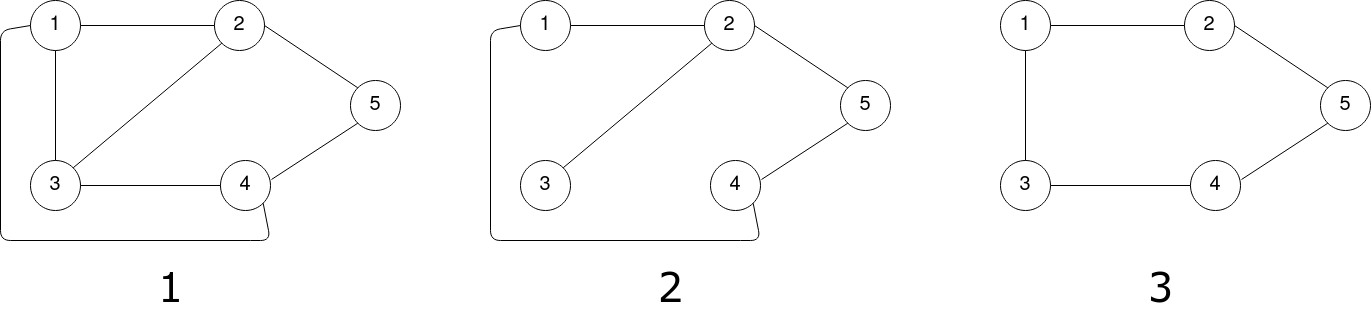
\includegraphics[scale=0.35]{files/1TreeEsempi.png}
    \caption{Nel grafo 1 è proposta un'istanza di grafo $G(V,E)$ non orientato. I grafi 2 e 3 rappresentano due suoi 1-tree di cui 3 è anche un circuito hamiltoniano.}
\end{figure}

\section{Calcolo del Lower Bound e Upper Bound}
Una semplice procedura per calcolare un 1-tree di costo minimo e generare quindi un \textbf{lower bound} al problema del TSP segue i successivi passi:
\begin{enumerate}
    \item Si calcoli l'MST $T$ sul grafo ottenuto da $G$ scartando il nodo prescelto $n$ e tutti gli archi incidenti su di esso. Sia $E_T$ l'insieme degli archi della soluzione trovata;
    \item Si aggiungano ad $E_T$ i due archi $(n,k)$ e $(n,h)$ a distanza minima tra quelli incidenti sul nodo $n$.
    \item Si restituisca l'1-tree $H = (V, E_H)$ con $E_H = E_T \cup \{(n,k),(n,h)\}$.
\end{enumerate}
Il costo della procedura appena proposta risulta dominato dal calcolo dell'MST, risolvibile facilmente con un algoritmo greedy come quello di  Kruskal in tempo $O(m\cdot log\: n)$. La selezione al passo 2 della coppia degli archi di costo minore è ottenibile invece con una semplice scansione degli archi $O(m)$.
\newline
Al costo di un maggiore sforzo computazionale si possono anche calcolare tutti gli 1-tree minimi variando la scelta del nodo $n$ tra tutti i $|V|$ nodi del grafo. Come lower bound complessivo si potrà in questo modo scegliere il migliore ottenuto, ovvero il più grande trovato.
\newline
Per quanto riguarda il calcolo e l'aggiornamento dell'\textbf{upper bound}, ricordiamo che questo si basa sull'identificazione di soluzioni ammissibili durante l'esecuzione dell'algoritmo. Una volta calcolato un 1-tree se questo risulta anche un circuito hamiltoniano, ossia ogni nodo presenta grado 2, si può aggiornare l'upper bound se presenta un costo minore di quello per ora trovato. All'inizio del procedimento l'upper bound sarà impostato a $ + \infty$. 

\section{Schema di Branch}
Ci occuperemo ora di mostrare come sarà partizionata la regione ammissibile $S$ in più sottoinsiemi. Se non siamo nel caso fortunato in cui la soluzione del rilassamento è un circuito hamiltoniano, tale soluzione sarà allora un 1-tree che contiene esattamente un sottocircuito. Dobbiamo introdurre una regola di suddivisione il cui scopo è impedire il formarsi nei nodi figli di tale sottocircuito. Indichiamo con: $\{(i_1, j_1), (i_2,j_2),...,(i_r,j_r)\}$ gli archi che compongo tale sottocircuito. Il primo nodo figlio verrà generato imponendo che l'arco $(i_1,j_1)$ non faccia parte della soluzione, ossia impostando $x_{i_{1}j_{1}} = 0$. Il secondo nodo figlio sarà ottenuto imponendo che sia presente l'arco $(i_1,j_1)$, ma sia assente l'arco $(i_2,j_2)$, ovvero impostando $x_{i_{1}j_{1}} = 1$ e $x_{i_{2}j_{2}} = 0$. Il procedimento continua in questo modo fino all' r-esimo figlio che avrà tutti i primi $r-1$ archi del sottocircuito e non conterrà l'ultimo, quindi $\forall k = 1,2,...,r-1 \:\:x_{i_{k}j_{k}} = 1$ e $x_{i_{r}j_{r}} = 0$.
\newpage
Ad ogni nodo saranno quindi associati due insiemi: 
\begin{enumerate}
    \item $E_0$ contente tutti gli archi che non devono essere considerati;
    \item $E_1$ contenente tutti gli archi che devono essere in soluzione.
\end{enumerate}
Naturalmente sarà anche necessario che $E_0 \cap E_1 = \emptyset$.
\newline
Per ogni figlio si dovrà quindi risolvere un sottoproblema del tipo $S(E_0, E_1)$ contenente tutti i cicli hamiltoniani formati sicuramente dagli archi in $E_1$ e privi degli archi in $E_0$.
Per il calcolo del lower bound di un sotto problema $S(E_0, E_1)$ si usa la stessa procedura analizzata nel paragrafo precedente imponendo però la presenza degli archi $E_1$ ed escludendo quelli in $E_0$ per il calcolo dell'MST e nella scelta dei 2 archi per il nodo $n$.
In particolare si risolverà sempre il problema dell'MST con l'algoritmo greedy di Kruskal, ma inizializzando l'insieme $E_T$ con gli archi in $E_1$ non incidenti sul nodo $n$, invece che impostarlo come insieme vuoto. Una volta fatto ciò durante l'esecuzione dell'algoritmo non dovranno essere presi in considerazione gli archi in $E_0$. Ottenuto l'albero di copertura $T$ a questi saranno aggiunti i migliori (con costo più basso) archi incidenti in $n$. Nel caso in cui $E_1$ contenesse tali archi saranno selezionati altrimenti si sceglieranno i migliori non presenti in $E_0$. 
\newline
Per il branching di un nodo interno, al sottocircuito $\{(i_1, j_1), (i_2,j_2),...,(i_r,j_r)\}$ individuato andranno tolti gli archi in $E_1$, che non possono non essere presenti nei figli che saranno generati. Una volta scremato l'insieme di archi si procederà alla stessa maniera.
\newline
Con questa regola di branching i nodi figli di un dato nodo continueranno ad essere sottoinsiemi della regione ammissibile del padre.

\section{Criteri di chiusura dei nodi}
Un nodo dell'albero di branch $P_i$ viene chiuso quando:
\begin{enumerate}
    \item $\hat{z} \leq LB(P_i)$, ossia quando il lower bound fornito è maggiore del migliore circuito hamiltoniano per ora trovato, in tal caso il nodo viene \textbf{chiuso per bound};
    \item non si riesce a calcolare un 1-tree per il nodo, non c'è soluzione ammissibile per il rilassamento, in tal caso il nodo sarà \textbf{chiuso per inammissibilità};
    \item l'1-tree generato dal rilassamento risulta essere un circuito hamiltoniano, il nodo verrà allora \textbf{chiuso per otttimalità}.
\end{enumerate}
Nell'ultimo caso delineato qualora il nodo presentasse anche un costo migliore e quindi minore dell'attuale soluzione trovata, questa verrebbe aggiornata.
\newline
Se alcuni nodi risultano aperti la scelta del prossimo nodo su cui fare Branch ricade su quello che presenta un Lower Bound minore, ossia quello che ci permette, in caso di ottimalità, di chiudere prima eventuali nodi aperti e terminare l'esecuzione. Un tale approccio viene detto \textbf{Best First}.

\section{Analisi dell'implementazione}
L'intero codice implementativo può essere visionato direttamente presso la pagina \href{https://github.com/LorenzoSciandra/TesinaOttimizzazioneCombinatoria}{GitHub} della tesina. Seguirà in questo paragrafo un'analisi delle scelte rilevanti compiute e uno sguardo sull'esecuzione degli algoritmi discussi su istanze medio/grandi di grafi.
\newline
Per quanto riguarda la struttura dati utilizzata abbiamo implementato il grafo e quindi anche l'1-tree che di volta in volta calcoliamo con delle \textbf{liste di adiacenze} realizzate con HashMap. Nello specifico il grafo è visto come un'insieme di nodi, che a loro volta contengono insiemi di archi. Entrambi questi insiemi sono stati realizzati con HashMap per rendere più efficiente il recupero dell'informazione. Questa scelta risulta la più conveniente dal punto di vista della complessità per i compiti che dobbiamo svolgere. Un'esplorazione completa del grafo, così come lo spazio necessario per la memorizzazione richiede complessità $O(n+m)$, mentre la scansione degli adicenti di un nodo risulta di costo minimo $O(|A(u)|)$, dove $A(u) = \{v \:|\: (u,v) \in E\}$.
\newline
Rispetto alla scelta di usare delle matrici di incidenza, risulta svantaggiato il controllo dell'esistenza di un arco nel grafo che richiede tempo $O(1)$ con le matrici di adiacenza e $O(|A(u)|)$ con le liste di adiacenza. Dato che quest'operazione non viene da noi mai eseguita, mentre risultano centrali l'operazione di scansione degli adiacenti di un nodo e dell'intero grafo, le liste di adiacenza si dimostrano ottime. Questi compiti richiedono infatti rispettivamente complessità $O(n)$ e $O(n^2)$ con una matrice di adiacenza. 
\newline
\newline
Tra le procedure più spesso eseguite troviamo sicuramente il calcolo del \textbf{Minimum Spanning Tree}, che viene ripetuto per ogni nodo dell'albero di Branch che andiamo a generare. Per tale calcolo abbiamo implementato l'algoritmo greedy proposto da Kruskal che presenta complessità ottima $O(m \cdot log\:n)$. Tale costo risiede principalmente nell'ordinamento decrescente iniziale degli archi, e nell'uso degli Mfset per controllare che un i-esimo arco possa essere incluso in soluzione con la certezza che non formi un ciclo. Ricordiamo che il Merge find set rappresenta una partizione di un insieme finito in sottoinsiemi disgiunti dette componenti o parti. Le operazioni ammesse permettono di controllare a quale componente appartiene un certo elemento e di unire due componenti diverse. Entrambe le operazioni presentano complessità $O(log\: n)$, dove $n$ rappresenta la cardinalità dell'insieme analizzato.
\newline
\newline
Per quanto riguarda l'individuazione del sottociclo all'interno di un 1-tree che non è un circuito hamiltoniano abbiamo usato una \textbf{Depht First search} con complessità $O(n+m)$. L'idea è usare un vettore di padri per evitare di visitare più volte i nodi del grafo e per tener traccia del padre di ogni nodo. Conclusa l'esplorazione in profondità del grafo, semplicemente partendo dal nodo candidato $n$ e procedendo con i vettori dei padri a ritroso, si individua il ciclo che ci servirà per il fare il Branch di un problema $P_i$.
\newline
\newline
La procedura centrale per la risoluzione del TSP è firmata \textit{branchAndBoundTSP()} e restituisce la migliore istanza della classe \textit{CicloHamiltoniano}, ossia quella con costo minore. In caso in cui non vi fosse un ciclo hamiltoniano nel grafo di partenza verrebbe restituito il grafo originale. Questo metodo richiama gli algoritmi sopra descritti e molte altre procedure di supporto al fine di gestire una lista di \textit{SubProblem} e terminando l'esecuzione non appena quest'ultima viene completamente svuotata grazie alla chiusura di tutti i nodi. \'E qui che risiede tutta la complessità della risoluzione del TSP simmetrico, questo metodo infatti richiama sottoprocedure polinomiali in tempo, ma il numero di \textit{SubProblem} che deve gestire può essere esponenziale.
\newline
La gestione dell'insieme dei SubProblem ancora aperti è stata realizzata con una coda di priorità \textbf{min-heap}, ossia con una struttura dati che presenta complessità $O(1)$ per leggere l'elemento con lower bound minore e $O(log\:n)$ per estrarre ed aggiungere un elemento.
\end{document}
